\section{Original Benchmark Results}
\label{sec:original-results}
\begin{table*}[t]
\centering\footnotesize
\caption{E1/E2/E6: archived grounding and evidence sufficiency at 6,000 surrogate tokens. Sufficiency uses the original declared-fact bookkeeping, not a universal accuracy bound.}
\label{tab:archive-context}
\setlength{\tabcolsep}{3.5pt}
\begin{tabular}{@{}lrrrrrrrrr@{}}
\toprule
Context & Top-1 & MRR & R@5 & Verif. & Distr@5 & Coverage & Suff. & Tokens & Cov./1k \\
\midrule
C0 & 0.000 & 0.000 & 0.000 & 0.000 & 0 & 0.100 & 0.000 & 407 & 0.247 \\
C1 & 0.789 & 0.866 & 1.000 & 0.000 & 10 & 0.252 & 0.000 & 1310 & 0.192 \\
C2 & 0.947 & 0.974 & 1.000 & 0.947 & 7 & 0.549 & 0.229 & 5193 & 0.106 \\
C3 & 1.000 & 1.000 & 1.000 & 1.000 & 4 & 0.761 & 0.514 & 5332 & 0.143 \\
C4 & 1.000 & 1.000 & 1.000 & 0.842 & 4 & 0.857 & 0.857 & 5290 & 0.162 \\
\bottomrule
\end{tabular}
\end{table*}

\begin{table*}[t]
\centering\footnotesize
\caption{E6: archived evidence sufficiency by task category. GRD identity; UNI units; RNG ranges; TOP topology; PRV provenance; ACT actions; SAF guards; REC recipes.}
\label{tab:archive-categories}
\setlength{\tabcolsep}{3.5pt}
\begin{tabular}{@{}lrrrrrrrr@{}}
\toprule
Context & GRD & UNI & RNG & TOP & PRV & ACT & SAF & REC \\
\midrule
C0 & 0.000 & 0.000 & 0.000 & 0.000 & 0.000 & 0.000 & 0.000 & 0.000 \\
C1 & 0.000 & 0.000 & 0.000 & 0.000 & 0.000 & 0.000 & 0.000 & 0.000 \\
C2 & 1.000 & 0.000 & 0.600 & 0.000 & 0.000 & 0.000 & 0.000 & 0.000 \\
C3 & 1.000 & 0.800 & 0.800 & 1.000 & 0.000 & 0.000 & 0.000 & 0.000 \\
C4 & 0.800 & 0.800 & 0.600 & 1.000 & 0.750 & 1.000 & 1.000 & 1.000 \\
\bottomrule
\end{tabular}
\end{table*}

\subsection{E1, E2 and E6: Resolution and evidence sufficiency}
Table~\ref{tab:archive-context} distinguishes locating a likely tag from carrying
enough facts for a checkable answer. C1 resolves 79\% of single-tag questions
but provides no explicit membership proof; C2 reaches 95\% top-1 with 23\%
task sufficiency. C3/C4 achieve perfect top-1 resolution under their scoped
resolver, yet context can omit a fact required for audit. Verifiable grounding
checks the membership evidence, not merely whether the ranked identifier equals
the gold identifier.

Table~\ref{tab:archive-categories} localises the archived treatment effects.
Typing supports identity and many range questions; unit/topology facts support
quantity reporting and impact tasks; state, guards and provenance support the
remaining operational categories. These categories were constructed around the
capabilities, so the block structure is evidence within the benchmark, not a
proof that every future task has one uniquely necessary layer.

\begin{figure*}[t]
\centering
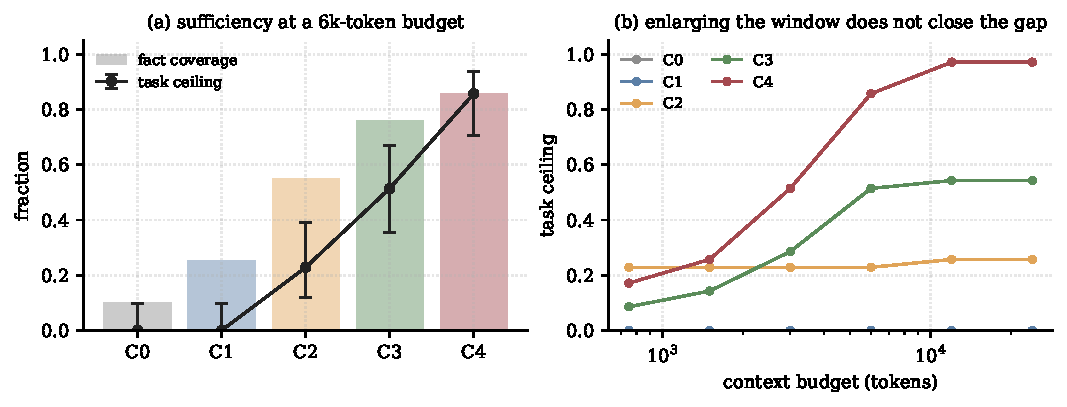
\includegraphics[width=0.94\linewidth]{../paper/figures/fig_ceiling.pdf}
\caption{Retained E2/E6 figure. The original axis term ``ceiling'' means declared-evidence sufficiency, not an unconditional LLM accuracy bound. Original conversion bookkeeping is preserved; audited R2 results are separate.}
\label{fig:archive-budget}
\end{figure*}
Increasing the budget from 750 to 24,000 tokens raises C2's archived sufficiency
from 0.229 to 0.257, versus 0.171 to 0.971 for C4. More space cannot reveal fact
kinds omitted by the selected projection, but can help a richer projection retain
them. This does not establish that a more complete OPC UA/AAS profile would
show the same plateau. At fixed budgets extra state, event and guard records
can displace measurements, motivating task-dependent retrieval.

\subsection{E3: Format costs and context economy}
\begin{table}[t]
\centering\footnotesize
\caption{E3: archived format costs. Formats do not preserve identical fact inventories; ratios mix content and syntax. R5 tests fidelity separately.}
\label{tab:archive-formats}
\setlength{\tabcolsep}{3.5pt}
\begin{tabular}{@{}lrr@{}}
\toprule
Format & Tokens & Ratio/CSV \\
\midrule
CSV & 2256 & 1.0 \\
NGSI-LD & 11233 & 5.0 \\
WoT TD & 18471 & 8.2 \\
Turtle & 45803 & 20.3 \\
OPC UA XML & 52324 & 23.2 \\
AAS JSON & 65929 & 29.2 \\
N-Triples & 179241 & 79.5 \\
JSON-LD & 145260 & 64.4 \\
\bottomrule
\end{tabular}
\end{table}

The archived CSV costs 2,256 surrogate tokens, OPC UA XML 52,324 and AAS JSON
65,929 (Table~\ref{tab:archive-formats}); N-Triples is substantially larger.
These figures describe emitted artefacts, not an intrinsic ranking of standards:
CSV carries fewer facts, projections differ and formatting affects the count.
An exchange format can be useful even if it is poor prompt material. The
engineering implication is to serve typed queries or selected evidence slices,
while R5 checks whether syntax-only comparisons preserve the graph. Billing
claims require the actual model tokenizer and repeated tool-schema overhead.

\subsection{E4 and E4b: Faults, false alarms and procedural checks}
\begin{table}[t]
\centering\footnotesize
\caption{E4: archived validator results on 84 faulty and 53 valid actions. Intervals are descriptive Wilson recall intervals.}
\label{tab:archive-guardrails}
\setlength{\tabcolsep}{3.5pt}
\begin{tabular}{@{}lrrrrr@{}}
\toprule
Tier & Caught & Recall & 95\% CI & Diag. & FPR \\
\midrule
G0 & 0/84 & 0.000 & [0.00,0.04] & 0.000 & 0.000 \\
G1 & 12/84 & 0.143 & [0.08,0.23] & 0.143 & 0.000 \\
G2 & 57/84 & 0.679 & [0.57,0.77] & 0.631 & 0.075 \\
G3 & 62/84 & 0.738 & [0.64,0.82] & 0.738 & 0.000 \\
G4 & 84/84 & 1.000 & [0.96,1.00] & 1.000 & 0.000 \\
\bottomrule
\end{tabular}
\end{table}

\begin{table}[t]
\centering\footnotesize
\caption{E4: detected counts by injected fault family. R1 audits raw family sets without gold-derived reclassification.}
\label{tab:archive-families}
\setlength{\tabcolsep}{3.5pt}
\begin{tabular}{@{}lrrrrr@{}}
\toprule
Family & $n$ & G1 & G2 & G3 & G4 \\
\midrule
F-ACC & 8 & 0 & 8 & 8 & 8 \\
F-CARD & 8 & 8 & 8 & 8 & 8 \\
F-DIM & 13 & 0 & 13 & 13 & 13 \\
F-ENUM & 4 & 4 & 4 & 4 & 4 \\
F-ILK & 3 & 0 & 0 & 0 & 3 \\
F-RANGE & 8 & 0 & 8 & 8 & 8 \\
F-REF & 12 & 0 & 12 & 12 & 12 \\
F-SCOPE & 5 & 0 & 0 & 5 & 5 \\
F-STALE & 4 & 0 & 0 & 0 & 4 \\
F-STATE & 7 & 0 & 0 & 0 & 7 \\
F-UNITSCALE & 4 & 0 & 4 & 4 & 4 \\
F-VALUE & 8 & 0 & 0 & 0 & 8 \\
\bottomrule
\end{tabular}
\end{table}

\begin{table}[t]
\centering\footnotesize
\caption{E4b: original unit-calculus procedural baseline (GP), not the equally informed R1 implementation.}
\label{tab:archive-procedural}
\setlength{\tabcolsep}{3.5pt}
\begin{tabular}{@{}lrrrr@{}}
\toprule
Tier & Recall & FPR & Scale & Behav. \\
\midrule
G2 & 0.679 & 0.075 & 0/4 & 0/22 \\
GP & 0.679 & 0.000 & 4/4 & 0/22 \\
G3 & 0.738 & 0.000 & 4/4 & 0/22 \\
G4 & 1.000 & 0.000 & 4/4 & 22/22 \\
\bottomrule
\end{tabular}
\end{table}

G2 detects 57 of 84 faulty proposals, but rejects four legal unit re-expressions.
G3 detects 62 without those false alarms, and G4 detects all 84
(Table~\ref{tab:archive-guardrails}). Literal unit comparison explains both
unnecessary rejection and incorrect diagnosis of scale errors. The family
breakdown (Table~\ref{tab:archive-families}) includes invalid references,
arguments/enumerations, access, ranges, dimension/scale, scope, guards, states,
staleness and unfaithful values. Behaviour/provenance families total 22 faults
in this designed corpus, not a frequency estimate for real incidents.

The original GP baseline supplies unit calculus but not full behaviour, guard
or observation models (Table~\ref{tab:archive-procedural}). It removes unit
false alarms but cannot show semantic validation outperforming equally informed
procedural rules. R1 supplies that comparison. Archived diagnosis also identifies
the injected scale family through gold-dependent reclassification; the revised
raw-family audit avoids that prediction-time label dependence.

\subsection{E5: Admissible calls and schema cost}
\begin{table*}[t]
\centering\footnotesize
\caption{E5: admitted write and command spaces; P and R are precision and recall against reference legality.}
\label{tab:archive-actions}
\setlength{\tabcolsep}{3.5pt}
\begin{tabular}{@{}lrrrrrrr@{}}
\toprule
Tier & Writes & Write P & Write R & Bits removed & Commands & Cmd P & Cmd R \\
\midrule
G0 & 71540 & 0.010 & 1.000 & 0.00 & 153 & 0.170 & 1.000 \\
G1 & 71540 & 0.010 & 1.000 & 0.00 & 153 & 0.170 & 1.000 \\
G2 & 190 & 0.937 & 0.251 & 8.56 & 81 & 0.321 & 1.000 \\
G3 & 755 & 0.940 & 1.000 & 6.57 & 81 & 0.321 & 1.000 \\
G4 & 710 & 1.000 & 1.000 & 6.65 & 26 & 1.000 & 1.000 \\
\bottomrule
\end{tabular}
\end{table*}

The reference enumerates 71,540 well-formed write triples and 153 command calls.
Only 710 writes and 26 commands are legal in its current state. G2 admits 190
writes because literal-unit restrictions exclude many legal re-expressions;
G3 admits 755 and G4 the 710 reference-legal writes. Table~\ref{tab:archive-actions}
reports admitted-set precision and recall. Uniform-call legality is a property
of this enumeration, not an estimate of an LLM's proposal distribution.

The write schema grows from 205 surrogate tokens at C0 to 981 at C2, 1,669 at
C3 and 2,317 at C4. Static enums and numeric limits can constrain generation,
but live-state facts in a cached schema expire. Cost is not assumed to be paid
only once: models may receive tools repeatedly, and refresh policies must be
documented. Decoder support and later validation jointly determine which calls
are impossible versus merely checked after generation.

\subsection{E7: Query execution instead of stuffing}
\begin{table}[t]
\centering\footnotesize
\caption{E7: hand-authored SPARQL execution costs, including query and result. Suff. marks the original stuffed context; query generation is not evaluated.}
\label{tab:archive-queries}
\setlength{\tabcolsep}{3.5pt}
\begin{tabular}{@{}lrrrr@{}}
\toprule
Task & Query+result & Stuffed & Ratio & Suff. \\
\midrule
UNI-05 & 153 & 5373 & 35.1 & yes \\
RNG-04 & 222 & 741 & 3.3 & no \\
TOP-02 & 79 & 5461 & 69.1 & yes \\
TOP-03 & 139 & 5172 & 37.2 & yes \\
ACT-04 & 84 & 5172 & 61.6 & yes \\
SAF-04 & 241 & 5172 & 21.5 & yes \\
PRV-04 & 287 & 5492 & 19.1 & yes \\
GRD-01 & 149 & 5501 & 36.9 & yes \\
\bottomrule
\end{tabular}
\end{table}

Eight hand-authored queries cost 79--287 tokens including results, against
741--5,501 for stuffed C4 contexts (Table~\ref{tab:archive-queries}). Savings
range from about 3.3 to 69 times in the saved JSON. RNG-04 checks plant-wide alarm violations;
its top-$k$ context is insufficient at all tested budgets, while a query returns
the needed aggregate. This concerns execution of an existing correct query, not
query generation, repairs, endpoint latency or access control. Parameterised
reviewed queries can expose this benefit without arbitrary graph access.

\subsection{E8 and E9: Naming and projection robustness}
\label{sec:e8}
\begin{table}[t]
\centering\footnotesize
\caption{E8: top-1 accuracy / wrong non-empty resolution across naming conventions. Wrong non-empty resolution is not calibrated model confidence.}
\label{tab:archive-naming}
\setlength{\tabcolsep}{3.5pt}
\begin{tabular}{@{}lrrrr@{}}
\toprule
Scheme & C1 & C1+decode & C2+decode & C4 \\
\midrule
mnemonic & 0.79/0.21 & 0.95/0.05 & 0.95/0.05 & 1.00/0.00 \\
opaque & 0.53/0.47 & 0.53/0.47 & 0.95/0.05 & 1.00/0.00 \\
kks & 0.89/0.11 & 0.89/0.11 & 0.95/0.05 & 1.00/0.00 \\
vendor & 0.42/0.58 & 0.42/0.58 & 0.95/0.05 & 1.00/0.00 \\
inconsistent & 0.84/0.16 & 0.63/0.37 & 0.95/0.05 & 1.00/0.00 \\
\bottomrule
\end{tabular}
\end{table}

\begin{table}[t]
\centering\footnotesize
\caption{E9: original neighbourhood (N) and routed (R) projection at 6,000 tokens. R2 uses a more conservative conversion-evidence audit.}
\label{tab:archive-routing}
\setlength{\tabcolsep}{3.5pt}
\begin{tabular}{@{}lrrrrr@{}}
\toprule
Context & Mode & Suff. & Coverage & Verif. & Tokens \\
\midrule
C3 & N & 0.514 & 0.761 & 1.000 & 5332 \\
C3 & R & 0.543 & 0.774 & 1.000 & 5341 \\
C4 & N & 0.857 & 0.857 & 0.842 & 5290 \\
C4 & R & 0.943 & 0.959 & 1.000 & 5345 \\
\bottomrule
\end{tabular}
\end{table}

Re-tagging changes identifiers but holds engineering facts fixed. Mnemonic
decoding reaches 95\% grounding on its native convention but varies by 53
percentage points across schemes. With misleading mnemonics it reaches 63\%
against 84\% without decoding. Explicit membership keeps the typed resolver
at 95\% and the graph resolver at 100\% for these perturbations
(Table~\ref{tab:archive-naming}). The original ``confidently wrong'' field means
a non-empty wrong resolution, not calibrated model confidence.

Original routed C4 projection raises declared sufficiency from 0.857 to 0.943
and verifiable grounding from 0.842 to 1.000 at nearly equal token cost
(Table~\ref{tab:archive-routing}). The router is a fixed lexicon, not a learned
policy or universal lower bound. R2's conversion audit changes sufficient-task
sets; the two findings must not be pooled as though the evidence definitions
were identical.